\documentclass[10pt]{beamer}

\usepackage{style-custom}


\title{Teoria del Gruppo di Rinormalizzazione in dinamica}
% \subtitle{Colloquio IV anno}
\author[Carmelo Mordini]{Carmelo Mordini}

% \institute[SNS]
% {
%   Scuola Normale Superiore\\
%   %University of Somewhere
%   }
\date{\small{Settembre 2014}}


% Delete this, if you do not want the table of contents to pop up at
% the beginning of each subsection:
\AtBeginSection[]
{
  \begin{frame}<beamer>{Outline}
    \tableofcontents[currentsection]%,currentsubsection]
  \end{frame}
}

% Let's get started


\begin{document}


%\beamertemplatenavigationsymbolsempty

\begin{frame}[plain]
\advance\textwidth2cm
\hsize\textwidth
\columnwidth\textwidth
  \titlepage
\end{frame}


\begin{frame}{Outline}
\transwipe[direction=270]
  \tableofcontents%[pausesections]
  % You might wish to add the option [pausesections]
\end{frame}

% Section and subsections will appear in the presentation overview
% and table of contents.
\section{Dinamica dissipativa}
\subsection{Equazioni dinamiche}

\begin{frame}{Equazioni dinamiche - I}

Vogliamo studiare la dinamica di un sistema vicino alla transizione di fase, e il modo in cui questo rilassa eventualmente all'equilibrio.

In un modello efficace (\emph{coarse-grained}) del nostro sistema, dobbiamo introdurre delle equazioni cinetiche che descrivano la dissipazione in modo fenomenologico.
\pause
\vskip10pt

\underline{Esempio classico}: moto browniano

\begin{equation*}
 m\ddot{\vec x} = \vec f(x) - \gamma m \dot{\vec x} + \vec \eta(t) \qquad \text{\footnotesize eq. di Langevin}
\end{equation*}

\vskip10pt
overdamping: $\rightarrow \quad \dot p  = -\gamma p + \eta(t)$

I coefficienti $\gamma$ ed $\eta$ riassumono in modo efficace l'interazione con il bagno termico.
\end{frame}

\begin{frame}{Equazioni dinamiche - II}

Generalizzo ad un sistema con hamiltoniana $\ham [q_i]$

 \begin{equation*}
%     \begin{cases}
%         \dot p_i = -\frac{\partial \ham}{\partial q_i} \equiv v_i\\
%         \dot q_i = \frac{\partial \ham}{\partial p_i} \equiv w_i 
%      \end{cases}
  \dot q_i = \Omega_{ij} \frac{\partial \ham}{\partial q_j} \equiv v_i
    \quad \longrightarrow \quad
    \dot q_i = v_i -\displaystyle \frac{\Gamma_i}{T} \frac{\partial \ham}{\partial q_i} + \zeta_i(t) 
%    \begin{cases}
%         \dot p_i = v_i -\frac{\Gamma_i}{T} \frac{\partial \ham}{\partial p_i} + \zeta(t) \\
%         \dot q = w_i
%      \end{cases}
  \end{equation*}

 \begin{itemize}
 \item<+-> $v_i$ mode-mode coupling fissato dall'hamiltoniana
 \item<+-> $\Gamma$ smorzamento: determina la scala di tempo di dissipazione dell'energia
 
 \item<+-> $\zeta$ rumore gaussiano locale e decorrelato
 \begin{flalign*}
  & \mean{\zeta_i(t)} = 0 \\
  & \mean{\zeta_i (t) \zeta_j (t')} = 2 D_i \ \delta_{ij}\  \delta(t-t') &&
 \end{flalign*}
 
 \end{itemize}

  
\end{frame}

\begin{frame}{Evoluzione della probabilità}
  Con le ipotesi date, la distribuzione di probabilità dello spazio delle fase evolve secondo l'equazione di Fokker - Planck
  
  \begin{equation*}
   \dt P + \sum_i \frac{\partial}{\partial q_i} \left[ v_i - \frac{\Gamma_i}{T} \frac{\partial \ham}{\partial q_i} - D_i \frac{\partial}{\partial q_i} \right] P = 0
  \end{equation*}
\begin{columns}
 \begin{column}{.5\textwidth}
  \begin{figure}
       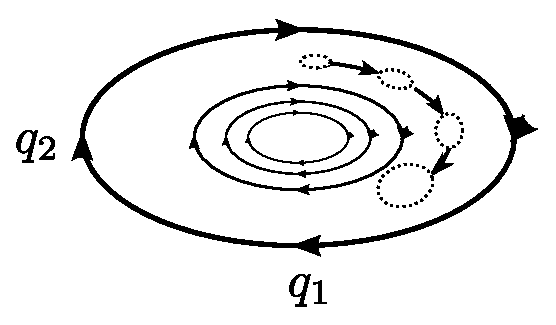
\includegraphics[width=.8\columnwidth]{pics/Oscillator_phase_portrait.eps}
      \end{figure}
  \end{column}
  \hfill
  \begin{column}{.4\textwidth}
   \begin{itemize}
    \item Hamiltonian velocity
    \item Damping
    \item Diffusion
   \end{itemize}
  \end{column}
\end{columns}

\vskip10pt
 per ottenere come soluzione stazionaria la distribuzione di equilibrio $P \propto e^{-\ham/T}$ è necessario soddisfare
 \begin{equation*}
  \Gamma_i = D_i \qquad \qquad \text{\footnotesize relazioni di Einstein}
 \end{equation*}

      
\end{frame}



\section{Funzioni caratteristiche della dinamica}
\subsection{Correlazione e risposta}

% \begin{frame}{Funzioni di correlazione e di risposta}
%   Date le soluzioni $q_i(t)$ si definisce
%  \begin{equation*}
%    C_{ij} (t-t') = \mean{q_i(t)\ q_j(t')}
%  \end{equation*}
%  o in trasformata di Fourier
%  \begin{equation*}
%    2\pi \delta (\omega + \omega') C_{ij}(\omega) = \mean{q_i(\omega)\ q_j(\omega')}
%  \end{equation*}
%  
%  Perturbo l'hamiltoniana con un piccolo campo esterno: $ \ham \rightarrow \ham - \sum_i q_i f_i(t)$\\
% La correzione lineare alle soluzioni si può scrivere come
% \begin{equation*}
%   \mean{q_i(t)} = \sum_j \int dt' \ G_{ij}(t-t')f_j(t') 
% \end{equation*}
% o in trasformata di Fourier
% \begin{equation*}
%   \mean{q_i(\omega)} = \sum_j G_{ij}(\omega)f_j(\omega) 
% \end{equation*}
% \end{frame}


\begin{frame}{Funzione di correlazione}
 Date le soluzioni $q_i(t)$ si definisce
 \begin{equation*}
   C_{ij} (t-t') = \mean{q_i(t)\ q_j(t')}
 \end{equation*}
 o in trasformata di Fourier
 \begin{equation*}
   2\pi \delta (\omega + \omega') C_{ij}(\omega) = \mean{q_i(\omega)\ q_j(\omega')}
 \end{equation*}
La forma di $C(\omega)$ dà informazioni sulla mutua correlazione dei modi $\{i,j\}$. In presenza di dissipazione, mi aspetto che \underline{l'autocorrelazione} $C_{ii}$ decada con una scala temporale tipica di ciascun modo.

\end{frame}

\subsection{Fluttuazione/dissipazione}
\begin{frame}{Funzione di risposta}
Perturbo l'hamiltoniana con un piccolo campo esterno: $ \ham \rightarrow \ham - \sum_i q_i f_i(t)$\\
La correzione lineare alle soluzioni si può scrivere come
\begin{equation*}
  \mean{q_i(t)} = \sum_j \int dt' \ G_{ij}(t-t')f_j(t') 
\end{equation*}
o in trasformata di Fourier
\begin{equation*}
  \mean{q_i(\omega)} = \sum_j G_{ij}(\omega)f_j(\omega) 
\end{equation*}

\pause
\begin{block}{Teorema di fluttuazione-dissipazione}
\begin{equation*}
  C_{ij}(\omega) = \frac{2}{\omega}\im G_{ij}(\omega)
\end{equation*}
  
\end{block}

\end{frame}

\subsection{Toy model}
\begin{frame}{Toy model: teoria di Van Hove}
Hamiltoniana di Ginzburg Laudau, in approssimazione gaussiana

\begin{equation*}
  \ham/T = \frac{1}{2} \sum_{k<\Lambda} (r_0 + ck^2)|\sigma_k|^2 = \frac{1}{2} \sum_{k<\Lambda}{G_0(k)}^{-1}\sigma_k \sigma_{-k} 
 \end{equation*}
 
\begin{equation*}
 \begin{cases}
 \displaystyle \dt{\sigma_k} = -\frac{\Gamma_k}{T}\frac{\partial \ham}{\partial \sigma_{-k}} + \zeta_k(t) = -\Gamma_k {G_0(k)}^{-1} \ \sigma_k + \zeta_k(t)  \\
 \mean{\zeta_k (t) \zeta_q (t')} = 2 \Gamma_k \ \delta_{-k,q}\  \delta(t-t') 
 \end{cases}
\end{equation*}

\pause
{\footnotesize
\begin{columns}
 \begin{column}{.5\textwidth}
   La soluzione in trasformata è\\
    \begin{flalign*}
     \sigma_k(\omega) = \frac{\zeta_k(\omega)}{\Gamma_k {G_0(k)}^{-1} - i\omega} &&
    \end{flalign*}
   e mediando sulle $\zeta$ calcolo
   \begin{flalign*}
    C_k(\omega) = \frac{2\Gamma_k}{\left(\Gamma_k {G_0(k)}^{-1}\right)^2 + \omega^2} &&
   \end{flalign*}

 \end{column}

 \begin{column}{.5\textwidth}
  Perturbo $\ham$ con $-\sum_k h_k(t) \sigma_{-k}$\\ La soluzione si sposta in
  \begin{flalign*}
   \mean{\sigma_k(\omega)} = \frac{\Gamma_k \ h_k(\omega)}{\Gamma_k {G_0(k)}^{-1} - i\omega} &&
  \end{flalign*}
  da cui
  \begin{flalign*}
   G_k(\omega) = \frac{\Gamma_k}{\Gamma_k {G_0(k)}^{-1} - i\omega} &&
  \end{flalign*}
 \end{column}

\end{columns}
}

\end{frame}

\begin{frame}{Toy model: teoria di Van Hove}
 \textbf{Remarks}
 \begin{itemize}
  \item Per $\omega = 0$ ritrovo la correlazione statica:\\
  $G(k,\omega = 0) = \int \frac{d\omega}{2\pi} \ C_k(\omega) = \mean{\sigma_{-k}\ \sigma_k} \equiv G_0(k)$
  \item Per ciascun $k$, $C_k$ è una lorentziana di larghezza
  \begin{equation*}
   \displaystyle \tau_k = \frac{G_0(k)}{\Gamma_k} \equiv \frac{1}{\Gamma_k}\ \frac{\xi^2/c}{1+\xi^2 k^2}\qquad \text{\footnotesize forma di scala}
  \end{equation*}
  
  \item Per $T = T_c \quad \left( \xi \to \infty\right) \qquad \Longrightarrow \displaystyle \tau_k \sim \frac{k^{-2}}{\Gamma_k}$
%     \begin{flalign*}
%      \tau_k \sim \frac{k^{-2}}{\Gamma_k} &&
%     \end{flalign*}
 \end{itemize}
 Il tempo di rilassamento \emph{diverge} alla transizione per i modi di alta lunghezza d'onda:\\
%  I modi di alta lunghezza d'onda (responsabili della transizione) hanno tempi di rilassamento divergenti:\\
    \centering \underline{critical slowing down}\\
Possiamo formulare un'\emph{ipotesi di scala dinamica}

\end{frame}



\section{Equazioni di RG}
\subsection{Rinormalizzazione delle equazioni dinamiche}
\begin{frame}{Rinormalizzazione delle equazioni dinamiche}
  Partendo dalle equazioni dinamiche per i modi $\sigma_k$, si applicano i due step già concettualmente definiti nel caso statico:
  \begin{itemize}
   \item[(i)] \emph{Coarse-graining}: elimino dal sistema i modi $\sigma_q$ con $\Lambda/s < q < \Lambda$.\\
   Ovvero, risolvo le equazioni dei $\sigma_q$, le sostituisco nel resto del sistema e medio sul rumore gaussiano $\zeta_q$ dei modi eliminati.
   \item[(ii)] \emph{Scaling \& renormalization}: i modi rimasti vengono riscalati sostituendo
   \begin{flalign*}
    \sigma_k(t) \longmapsto s^{1-\eta/2}\ \sigma_{sk}(s^{-z}t) &&%\Leftrightarrow \sigma_k(\omega) \mapsto s^{1-\eta/2 + z}\ \sigma_{sk}(s^z\omega)&&
   \end{flalign*}

  \end{itemize}

Infine, con il cambio di variabili $\{ t' = s^{-z} t\ ;\ k' = sk \}$\\
si portano le equazioni nella forma di partenza, trovando la legge di trasformazione nello spazio dei parametri allargato $\mu = (v,\ \Gamma,\ \mu_\ham)$. 

\end{frame}

\subsection{Trasformazione delle funzioni}
\begin{frame}{Trasformazione delle funzioni}
% Dopo la trasformazione $\Rightarrow$ le quantità medie dipendenti dai modi che non ho eliminato \underline{rimangono invariate} (non dipendono dalle variabili nel blocco) ed hanno la stessa forma funzionale (la forma delle equazioni è la stessa) [SCRIVILO MEGLIO]
La trasformazione lascia invariate le medie dei modi di alta lunghezza d'onda 
\begin{flalign*}
 \mean{\sigma_k(\omega)\ \sigma_q(\bar\omega)}_\mu = \mean{\sigma'_{k'}(\omega')\ \sigma'_{q'}(\bar\omega')}_{\mu'}  &&
\end{flalign*}
%  \begin{equation*}
%  \begin{cases}
%   \mean{\sigma_k(\omega)\ \sigma_q(\bar\omega)}_\mu = \mean{\sigma'_{k'}(\omega')\ \sigma'_{q'}(\bar\omega')}_{\mu'} \\
%   \sigma'_{k'}(\omega') = s^{1-\eta/2 + z}\ \sigma_{sk}(s^z\omega) \\
%  \end{cases}
%  \end{equation*}

% {\footnotesize
%  \begin{flalign*}
%   & \mean{\sigma_k(\omega)\ \sigma_q(\bar\omega)}_\mu = s^{2-\eta + 2z}\ \mean{\sigma_{sk}(s^z\omega)\ \sigma_{sq}(s^z \bar\omega)}_{R_s \mu} \\
%   & 2\pi \delta(\omega + \bar\omega)\ C(k,\omega,\mu) = 2\pi \delta(s^z(\omega + \bar\omega))\ s^{2-\eta+2z} C(sk,s^z\omega,R_s\mu) &&
%  \end{flalign*}
% }
\begin{block}

\vskip-10pt
\begin{align*}
 & C(k,\omega,\mu) = s^{2-\eta+z}\ C(sk,s^z\omega,R_s\mu)  \\
 & G(k,\omega,\mu) = s^{2-\eta}\ G(sk,s^z\omega,R_s\mu)
\end{align*}

\end{block}
\pause
Al punto critico corrispondente alla transizione di fase, il sistema viene portato da RG in un punto fisso stabile $\mu^*$.

N.B. è necessario che la parte statica dei parametri $\mu_\ham^*$ sia un punto fisso stabile del sistema in equilibrio \emph{(static fixed point)}
\begin{flalign*}
 \begin{cases}
  G(k,\omega,t) = \xi^{2-\eta}\ g(\xi k,\xi^z \omega) \\
  \tau_k(t) = \xi^z\ f(\xi k)\\
  \xi \sim t^{-\nu}
 \end{cases}
 \qquad \text{Si trovano le forme di scala} &&
\end{flalign*}
\end{frame}


\section{Modelli dinamici}
\subsection{Time Dependent Ginzburg Landau}
% \begin{frame}<beamer>{Outline}
%     \tableofcontents[currentsection,currentsubsection]
%   \end{frame}
\begin{frame}{TDGL}
 \transwipe[direction=270]
 \setbeamercovered{invisible} 
 \begin{equation*}
  \ham/T = \frac{1}{2} \sum_{k<\Lambda} (r_0 + ck^2)|\sigma_k|^2 %+ u \mathcal{V}% = \frac{1}{2} \sum_{k<\Lambda}{G_0(k)}^{-1}\sigma_k \sigma_{-k} 
 \end{equation*}
 \begin{itemize}
  \item[(i)]<+-> senza i termini di mode-mode coupling, le equazioni per i $\sigma_q$ sono disaccoppiate dal resto -- è sufficiente eliminarle
  \item[(ii)]<+-> sostituisco nelle rimanenti $ \left \{\sigma_k(\omega) \mapsto s^{1-\eta/2 + z}\ \sigma_{sk}(s^z\omega)\ ; \ \omega' = s^{z} \omega\ ;\ k' = sk \right\} $
 \end{itemize}
\only<1>
{
\begin{equation*}
  \begin{cases}
   \displaystyle -i\omega \sigma_k = -\Gamma_k(r_0 + ck^2)  \ \sigma_k + \zeta_k(\omega)\\
   \mean{\zeta_{-k}(\omega)\ \zeta_k(\bar\omega)} = 2\Gamma_k\ 2\pi \delta(\omega + \bar\omega)\\
   \end{cases}
\end{equation*}
}
\only<2->
{
\begin{equation*}
 \begin{cases}
    \displaystyle -i\omega' \sigma_{k'} = -s^{z-2}\ \Gamma_{k'/s}(s^2 r_0 + c{k'}^2)  \ \sigma_{k'} + s^{\eta/2 -1}\zeta_{k'/s}(s^{-z}\omega') \\
    \mean{\zeta'_{-k'}(\omega')\ \zeta'_{k'}(\bar\omega')} = 2 \Gamma'_{k'}\ 2\pi \delta(\omega' + \bar\omega')
   \end{cases} 
\end{equation*}
}
\visible<3>{
 \begin{itemize}
  \item[(iii)] definisco i nuovi parametri in modo da riportare le equazioni nella forma di partenza
 \end{itemize}
 
 \begin{equation*}
  \begin{cases}
   \zeta'_q(\omega) = s^{\eta/2 -1} \zeta_{q/s}(s^{-z}\omega) \\
   \Gamma'_q = s^{z+\eta-2} \Gamma_{q/s}\\
   r_0' = s^{2-\eta} r_0 \\
   c' = s^{-\eta} c
  \end{cases}
 \end{equation*}
 }
\end{frame}

\begin{frame}{TDGL - ruolo delle leggi di conservazione}
 Ho ritrovato la legge di trasformazione nota da RG statico.
 
 Fisso i parametri di $\ham$ sul punto fisso stabile statico:
 \begin{flalign*}
  & \text{Per} ~d> 4 \Rightarrow \eta = 0; \ (r_0^* = 0,\ c^*=1)  &\text{\footnotesize punto fisso gaussiano}\\
  & \text{Per} ~d< 4 \Rightarrow \eta = 0; \ (r_0^* \neq 0,\ u^* \neq 0) &\text{\footnotesize punto fisso di Wilson-Fisher}&&
 \end{flalign*}
 
 La forma di $\Gamma_k$ determina l'esponente critico dinamico: $\Gamma_k \approx \Gamma + \gamma k^2 + O(k^4)$

 \begin{itemize}
  \item[a)] $\Gamma \neq 0$: nelle equazioni dei modi con $k\to 0$ mantengo $\Gamma_k = \Gamma$\\
    $\Gamma' = s^{z-2} \Gamma$ ~ ha un punto fisso non banale se $z=2$
  
  \item[b)] $\Gamma = 0$: questo è fissato in un sistema in cui lo spin totale è conservato; la legge per il parametro $\gamma$ è\\
  $\gamma' = s^{z-4} \gamma$ ~ che ha un punto fisso non banale se $z=4$
 \end{itemize}
 
\end{frame}

\subsection{Isotropic ferromagnet}
\begin{frame}{Interazioni ferromagnetiche}
La dinamica degli spin è quella di precessione in un campo magnetico
\begin{flalign*}
\begin{cases}
\displaystyle  \dt{ \vec \sigma} = \lambda\  \vec \sigma \times \vec B(x) \\
\displaystyle \vec B(x) =  -\frac{\delta \ham}{\delta \vec \sigma(x)} = \vec h(x) + \nabla^2 \vec\sigma
\end{cases} &&
\end{flalign*}
Questo è un termine di mode-mode coupling nelle equazioni dinamiche per le componenti $\vec\sigma_{k}$

\begin{flalign*}
  &\displaystyle \vec v_k = \lambda L^{-d/2} \ \sum_{q} \vec \sigma_{k-q} \times (\vec h_q - q^2 \vec\sigma_q) \\
  & \dt{ \vec \sigma_k} = \vec v_k -\gamma k^2 \frac{\partial \ham}{\partial \vec \sigma_{-k}} + \vec \zeta_k(t) &&
\end{flalign*}
\end{frame}

\begin{frame}{Interazioni ferromagnetiche}
 Partendo dal punto fisso stabile del TDGL
 \begin{flalign*}
  &\mu_0^* = (\lambda = 0,\ \gamma,\ r_0^*,\ u^*)\\
  &\eta = 0,\ z=4 &&
 \end{flalign*}
Applico lo step (ii) ed osservo come trasforma $v_k$.\\ Ho $\lambda' = s^{z-1-d/2}\  \lambda = s^{3-d/2}\ \lambda\quad \Longrightarrow \quad \mu_0^*$ ~stabile per $d>6$
\end{frame}

\begin{frame}{Punto fisso per $d<6$}
 Con la procedura familiare, per $d= 6-\eps$, cerco un punto fisso stabile sviluppando ad $O(\eps)$ attorno al punto fisso gaussiano:

 \begin{equation*}
 \begin{cases}
   r_0 = u = 0 \\
   \lambda' = s^{z-4+\eps/2}\ \lambda \\
   \gamma' = s^{z-4}\ \gamma \left( 1 + \frac{1}{3} (\lambda/\gamma)^2 K_6 \ln s\right); \quad \tilde\lambda = \lambda/\gamma
  \end{cases}
 \end{equation*}
 
 \begin{flalign*}
  &\tilde\lambda' = s^{\eps/2} \tilde\lambda \left( 1 - \frac{1}{3} \tilde\lambda^2 K_6 \ln s\right) \quad\Rightarrow\quad 
  \begin{cases}
   \tilde\lambda^* = \pm \left( \frac{3\eps}{2K_6}\right)^{1/2}\\
   z= 4-\eps/2 = 1+d/2
  \end{cases} &&
 \end{flalign*}
\end{frame}

\begin{frame}{Conclusioni}
 \begin{itemize}
  \item<+-> La dinamica di un sistema vicino alla transizione è determinata dai modi di alta lunghezza d'onda: possiamo formulare un'\emph{ipotesi di scala dinamica}, per la quale i tempi di rilassamento divergono a causa della lunghezza di correlazione. RG permette di trovare la forma di scala $\tau_k \sim \xi^z \sim t^{-\nu z}$
  \item<+-> Per una stessa classe di universalità statica $(n,d)$ il comportamento critico è fortemente influenzato dal modello dinamico scelto: elementi come leggi di conservazione o accoppiamento tra i modi modificano le equazioni per il punto fisso ed i corrispondenti esponenti critici.
 \end{itemize}

\end{frame}

\end{document}


% % % All of the following is optional and typically not needed.
% % \appendix
% % \section<presentation>*{\appendixname}
% % \subsection<presentation>*{For Further Reading}
% % 
% % \begin{frame}[allowframebreaks]
% %   \frametitle<presentation>{For Further Reading}
% % 
% %   \begin{thebibliography}{10}
% % 
% %   \beamertemplatebookbibitems
% %   % Start with overview books.
% % 
% %   \bibitem{Author1990}
% %     A.~Author.
% %     \newblock {\em Handbook of Everything}.
% %     \newblock Some Press, 1990.
% % 
% % 
% %   \beamertemplatearticlebibitems
% %   % Followed by interesting articles. Keep the list short.
% % 
% %   \bibitem{Someone2000}
% %     S.~Someone.
% %     \newblock On this and that.
% %     \newblock {\em Journal of This and That}, 2(1):50--100,
% %     2000.
% %   \end{thebibliography}
% % \end{frame}
% 
% \end{document}
